\documentclass{article}
\usepackage[utf8]{inputenc}
\usepackage{graphicx}
\usepackage{amsmath}
\usepackage[citestyle=authoryear, backend=bibtex,
natbib=true]{biblatex}
\addbibresource{refs}

\title{V1 Modelling - Early Model Results}
\author{Ben Selby}
\date{August 12th, 2014}

\begin{document}

\maketitle

\section{Introduction}

In the effort to model the receptive fields of macaque primary visual cortex it is a good idea to first understand and model some of the individual variables of the receptive field. This allows some variables to be separated while others can be combined if they are found to be correlated. The goal of the model is to produce physiologically accurate responses to stimuli. In an attempt to start this process three variables of the V1 receptive field have been selected for modelling. They are orientation, spatial frequency, and contrast saturation. These are well studied properties of V1 with large datasets. Replicating these individual datasets (in this case, three figures from three journal articles) creates a first approximation to a V1 simple cell which may be integrated and extended to a model neuron population later. 

\section{Methods}

The basic receptive field for all three models is a 2D Gabor filter as used in many other models of V1. Gabor filters were shown by \citet{jp87} as an effective model of cat striate cortex receptive fields. The equation for a Gabor filter is as follows:

\begin{equation}
\begin{split}
\begin{matrix}
g(x,y) = {1 \over 2\pi \sigma_x \sigma_y}\exp{({-x'^2 \over 2\sigma_x^2} - {y'^2 \over 2\sigma_y^2})
}\cos{(kx'-\phi)} \\
x' = x\cos\theta - y\sin\theta \\
y' = x\sin\theta + y\cos\theta
\label{gabor_eq}
\end{matrix}
\end{split}
\end{equation}

where $\sigma_x$ and $\sigma_y$ are the standard deviations of the Gaussian envelope, $\theta$ is the preferred orientation, $k$ is the preferred spatial frequency, and $\phi$ is the phase offset. For convenience an arbitrary filter size of 25x25 pixels was selected. This receptive field size can later be parameterized for population models of V1. The 2D Gabor filter was then element-wise multiplied by the input image an the result was summed. This provided an input drive $J$ which was then passed into a LIF nonlinearity as presented in equation \ref{LIF} below:

\begin{equation}
\begin{matrix}
a = G[\alpha J + J_{bias}] \\ 
G[J] = {1 \over \tau_{ref} - \tau_{RC}\ln{(1 - 1/J)} } 
\label{LIF}
\end{matrix}
\end{equation}

where $a$ is the activation or firing rate of the neuron in spikes per second, $\alpha$ is a current gain, and $J_{bias}$ is a current bias. By optimizing over these Gabor function and LIF parameters it will be demonstrated that 2D Gabor functions will be effective in modelling receptive fields of V1 neurons in all three figures.

\subsection{Orientation Selectivity}

Orientation selectivity in V1 neurons was first identified by \citet{hw59} in cats. \citet{devalois82} present orientation tuning curves for macaque V1 cells, some of which are shown in figure \ref{fig:otuning}. Orientation tuning information was attained by moving lines and gratings across the visual field while recording spike rates from individual V1 neuron. Figure \ref{fig:otuning}C is the target figure for reproduction. It shows a simple cell which is bidirectionally tuned, responding to lines moving in two opposite directions. This figure was selected because it is considered ``close to the average for [the] whole cell population'' \citep{devalois82}. V1 cells show large variation of orientation bandwidth, with some cells responding to as narrow as 10 degrees while others show no orientation preference at all. 

The orientation receptive field of the V1 simple cell was modelled as a 2D Gabor function, as described in equation \ref{gabor_eq}. The input images were single white bars on black backgrounds of fixed width and varying orientation. The input images were normalized to contain intensity values of 0-1. A least-squares curve fitting operation was performed, optimizing over the parameters $\sigma_x$, $\sigma_y$, $\theta$, $k$, $\phi$, $\alpha$, $J_{bias}$, and $\tau_{RC}$. Contrast across input images was fixed at 100\%.

\begin{figure}[h]
\begin{center}
\includegraphics[width=5.25in]{figures/orientation-responses.png}
\caption{4 different V1 cell orientation responses. C) shows a simple cell response and is the target figure for reproduction here. \cite{devalois82}}
\label{fig:otuning}
\end{center}
\end{figure}

\subsection{Spatial Frequency Selectivity}
V1 neuron firing varies with the spatial frequency of stimuli. \citet{foster85} presents various spatial frequency tunings evident in V1. Figure \ref{fig:sftuning} shows the most common tunings. Figure \ref{fig:sftuning}A is the target for reproduction here because it is the most common amongst the V1 neurons recorded - 91\% of neurons in V1 demonstrated this bandpass type of firing. Gratings of fixed orientation and varying spatial frequency were presented and the neuron responses were recorded. 

Again, the receptive field was modelled as a 2D Gabor function. Input images were sinusoidal gratings of fixed orientation and varying spatial frequency. Neuron spatial frequency selectivity was reported in terms of number of cycles per degree of visual angle. Because the model neuron's receptive field size is arbitrary, the entire filter size was defined as 1 degree. The spatial frequency of test images was then considered the number of cycles present in the 25x25 image. A least-squares curve fitting operation was performed, optimizing over the parameters $\sigma_x$, $\sigma_y$, $k$, $\phi$, $\alpha$, $J_{bias}$, and $\tau_{RC}$. $\theta$ was fixed at 90 degrees, resulting in vertical line grating patterns as in the original figure. Contrast across input images was fixed at 100\%.

\begin{figure}[h]
\begin{center}
\includegraphics[width=5.05in]{figures/spatial-freq-tuning.png}
\caption{ V1 neuron response to varying stimulus spatial frequency. A) is the target figure for reproduction here. \cite{foster85}}
\label{fig:sftuning}
\end{center}
\end{figure}

\subsection{Contrast Saturation}

\citet{carandini97} and others before them show that V1 neurons exhibit \emph{response saturation} to contrast. Figure \ref{fig:con_saturation}B shows this and is the third target figure for reproduction. In this figure the size of change in spike rate decreases with increasing contrast. Using a linear model of the receptive field would result in linear scaling of response with contrast. Thus, in addition to the Gabor receptive field a contrast normalization was used, as specified by the following equation:

\begin{equation}
J_{norm} = J { c^n \over \sigma^n + c^n}
\end{equation}

where $J$ is the driving current from the Gabor receptive field, $c$ is the contrast of the image (calculated as the difference of the highest and lowest intensities divided by their sum), and $\sigma$ and $n$ are curve-fitting parameters. It is then $J_{norm}$ which is passed into the LIF nonlinearity to produce a spike rate. 

\begin{figure}[h]
\begin{center}
\includegraphics[width=4.95in]{figures/contrast-saturation.png}
\caption{ V1 neuron response to varying stimulus spatial frequency. B) is the target figure for reproduction here. \cite{carandini97}}
\label{fig:con_saturation}
\end{center}
\end{figure}

A least-squares curve fitting operation was performed, optimizing over the parameters $\sigma_x$, $\sigma_y$, $k$, $\phi$, $\alpha$, $J_{bias}$, and $\tau_{RC}$. $\theta$ was fixed at 90 degrees, resulting in vertical line grating patterns as in the original figure. Contrast across input images was fixed at 100\%.

\section{Results}
Figure \ref{fig:oresult} shows the result of the orientation selective neuron model, and figure \ref{fig:opolar} shows the same result plotted in polar co-ordinates as in the original figure. Figure \ref{fig:sfresult} shows the result of the spatial frequency selective neuron model. Figure \ref{fig:cresult} shows the result of the contrast saturation neuron model. Figure \ref{fig:cnonorm} shows the result of the contrast saturation model without contrast normalization. Unfortunately \LaTeX will not cooperate and put the figures where I would like them to be. 

\begin{figure}[h]
\begin{center}
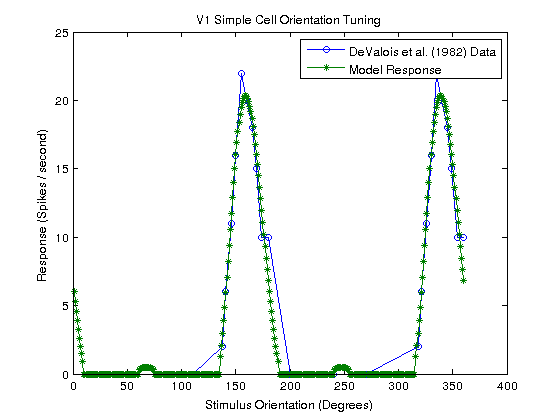
\includegraphics[width=4.75in]{figures/orientation_tuning_full.png}
\caption{Result of the orientation selectivity model.}
\label{fig:oresult}
\end{center}
\end{figure}

\begin{figure}[h]
\begin{center}
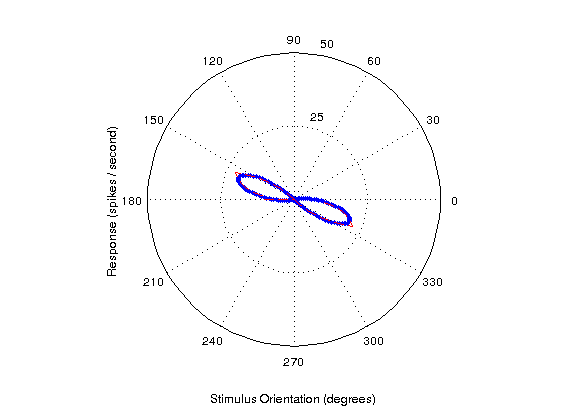
\includegraphics[width=4.75in]{figures/orientation_neuron_polar.png}
\caption{Result of the orientation selectivity model in polar coordinates.}
\label{fig:opolar}
\end{center}
\end{figure}


\begin{figure}[h]
\begin{center}
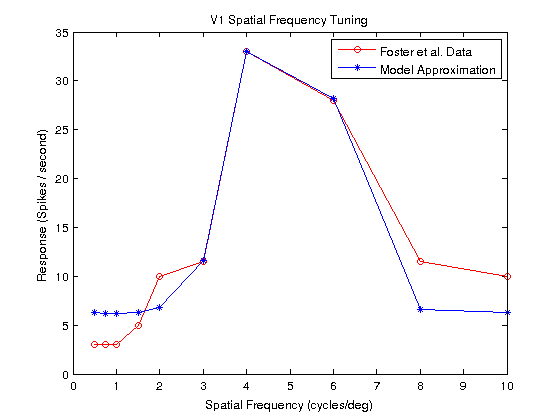
\includegraphics[width=4.75in]{figures/sfreq_tuning.png}
\caption{Result of the spatial frequency selectivity model.}
\label{fig:sfresult}
\end{center}
\end{figure}

\begin{figure}[h]
\begin{center}
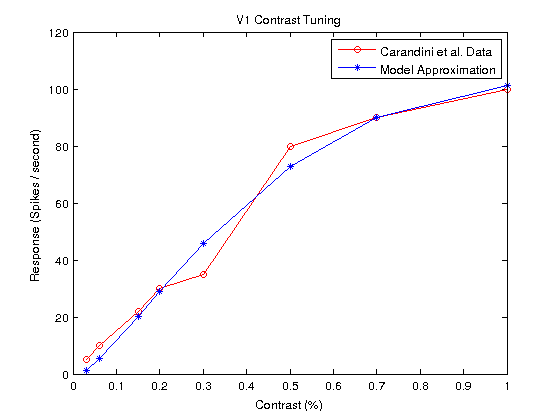
\includegraphics[width=4.75in]{figures/contrast_tuning.png}
\caption{Result of the contrast saturation model with normalization.}
\label{fig:cresult}
\end{center}
\end{figure}

\begin{figure}[h]
\begin{center}
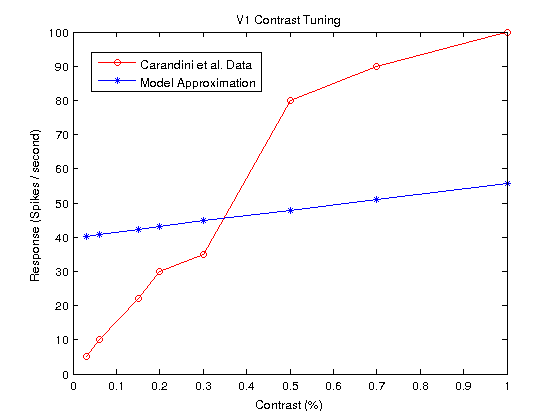
\includegraphics[width=4.75in]{figures/contrast_tuning_no_norm.png}
\caption{ Result of the contrast saturation model without normalization.}
\label{fig:cnonorm}
\end{center}
\end{figure}

\section{Discussion}
All three models demonstrate good fidelity to the figures which they reproduce. In each the general trend of the curve is matched, including all important features of each tuning curve. 

\subsection{Orientation Tuning}
In the case of the orientation figure, the resulting neuron appears to be cosine-tuned and responds in both directions (which in this figure corresponds to opposite directions of motion, a variable which was not simulated). It is interesting that there is a minor raise in firing at orientations orthogonal to the preferred direction. These raises could likely be smoothed out by specifying more zero-points in the optimization target data. However, \citet{devalois82} present other neurons which exhibit exactly this sort of orthogonal secondary firing mode. This may indicate that the current Gabor-LIF model may be suitable for producing other modes of neuron orientation tuning.

\subsection{Spatial Frequency Tuning}
The general curve of the spatial frequency model closely matches that of the figure. At peak response the model is identical to the data. At non-preferred frequencies the firing rate is slightly off - too high at low frequencies and too low at high frequencies. Like the orientation model, the neuron exhibits cosine tuning due to the way the input drive is calculated (element-wise multiplication and sum), which is analogous to a vector dot product. This cosine tuning results in a symmetric tuning curve and thus will not perfectly match the asymmetric curve of the data. It is important to note that the data presented is the recording from a single neuron, so it is likely that there is significant variability in the firing reported. It is also possible that there is some long-term potentiation/sensitization as a result of the continued stimulation of the neuron which results in the higher firing rate at higher frequencies. If not, this could be addressed by adding a sigmoid-like function which could elevate firing at higher spatial frequencies.

\subsection{Contrast Saturation}
Figure \ref{fig:cresult} shows that when contrast normalization is included in the model the data curve is fit quite well - the model demonstrates the characteristic response saturation with increasing contrast. When no normalization is included (figure \ref{fig:cnonorm}) the result is much worse - there is no saturation demonstrated. It is possible that another optimization method would produce a better fit without the normalization - this may be worth exploring when future models become increasingly complicated. The model was tested for a variety of fixed spatial frequencies and orientations and performed the same in every case - these variables are properties of the Gabor function and do not affect the response saturation. 

\subsection{Other Sources of Error}
One source of error for all three models is the extraction of data by eye from the original figures. This certainly introduces minor variances in the data a which the models are fit, and may explain the more minor apparent nonlinearities in the data. 

\subsection{Future Work}
All three studies made use of moving stimuli - DeValois et al. and Foster et al. used stationary stimuli for \emph{some} trials. This is an important distinction because it is known that V1 neurons are receptive to both direction of motion and temporal frequency. This would involve extending the Gabor receptive field to a third, time dimension. 

Normalization such as that used in the contrast saturation model has been proposed as a canonical neural computation which appears in many other neural models. Thus optimizing these parameters to fit neurons is a good exercise as similar curves will likely occur elsewhere, such as in contour integration and cross-orientation inhibition. 

Integrating the three results should be straightforward because all three are based around Gabor-LIF receptive fields. Adding the variables $k$ and $\theta$ to the optimization will expand the variable space to be searched over, so curve fitting will likely be more difficult. It will also be necessary to have a more complete set of physiological data to fit the parameters. Such a neuron can then be used in populations to model orientation column activity for instance. 

As a first approximation the Gabor-LIF-normalization model should be sufficient in modelling the major receptive fields of orientation, spatial frequency, and contrast saturation with a small set of variables. This model is fairly simple and thus should be easily extensible. Extending the Gabor receptive field into the time dimension sensitivity to direction of movement and temporal frequency will be added. Additional normalization fields among neighbouring neurons could be a good model of contour integration. The individual neuron models should be easily integrated into neurons for larger populations. 

\printbibliography

\end{document}
